\documentclass{article}
\usepackage{graphicx}

\title{A Common Yet Unknown Problem-Solving Technique: States}
\author{William Gvozdjak}

%% \blurb{Take a moment to read the following problem: ``I'm flipping a fair coin repeatedly. I'll keep flipping it until I reach a sequence of 3 consecutive flips that are HT. On average, how many times will I flip the coin?''}

\begin{document}

\maketitle
Take a moment to read the following problem:

``I'm flipping a fair coin repeatedly. I'll keep flipping it until I reach a sequence of 3 consecutive flips that are HT. On average, how many times will I flip the coin?''

At first glance, this problem seems really difficult: how are we supposed to find the average number of times that I'll flip the coin? In reality, if you know the right technique, this question becomes a simple problem of algebra.


First, we define each \textbf{state}: possible positions to be at in terms of the flips. Our first state, $1$, is the ``null'' state: there have been no flips that contribute to the desired HT. This is both at the start of the sequence of flips, and also at any time where the last flip was a T (this is because if the last flip was a T, we essentially are restarting, as we can't use that T to create an HT sequence). Then, we also have the state $2$, for when the last flip was an H. Notice that it doesn't matter what flips were prior to that H: the expected number of flips to reach HT will be the same no matter what flips were before that H. Finally, we have the state $3$, where the last two flips are HT: this is the desired state.

Now, define $a_i$ to be the expected number of flips to reach HT from the state $i$. First, note that we clearly have $a_3=0$: we're starting at the state HT, so we've already reached HT!

Consider state $2$ (we currently have H). There's a $\frac{1}{2}$ probability that we'll reach an HT from there (i.e., flip a T in the next flip). Therefore, we know that there's a $\frac{1}{2}$ probability that the expected number of flips to reach HT is $a_3+1$ (note that we must add $1$ to account for the one flip that we must use to reach state $3$). But there's also a $\frac{1}{2}$ probability that we flip an H in the next flip, which simply returns us to state $2$. Hence, we have
\[a_2=\frac{1}{2}(a_3+1)+\frac{1}{2}(a_2+1).\]
Finally, consider state $1$ (we currently either have nothing or T). If we flip an H, then we move to state $2$, and if we flip a T, we stay at state $1$. Therefore, we know that
\[a_1=\frac{1}{2}(a_2+1)+\frac{1}{2}(a_1+1).\]
Notice that we are looking for the value of $a_1$, as we want to find the expected number of flips necessary to reach HT from a state consisting of no flips.

We therefore have the following system of equations:
\begin{align*}
a_1&=\frac{1}{2}(a_2+1)+\frac{1}{2}(a_1+1) \\
a_2&=\frac{1}{2}(a_3+1)+\frac{1}{2}(a_2+1) \\
a_3&=0.
\end{align*}
But this is simply a system of $3$ linear equations with $3$ variables -- it's just an algebra problem! We can solve these three equations just as we would with any other system of linear equations, and we'd find that $a_1=\boxed{4}$.

\begin{center}
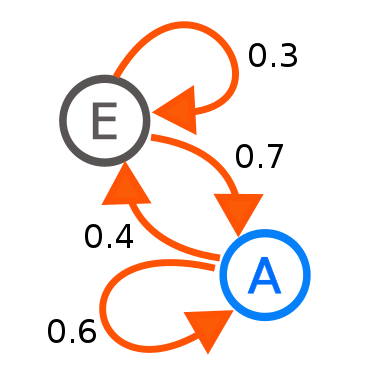
\includegraphics[scale=0.38]{images/finite_state.png}
\end{center}

In summary, states is a powerful technique that can be used to reduce seemingly difficult counting problems into matters of simple algebra and arithmetic. But also remember that this article just brushed the surface of states: states can be used to solve many different types of problems, from problems like the above one to walks on a grid. States are also an introduction to a more advanced topic known as \textbf{Markov chains} -- if you found this interesting, I highly recommend you explore and learn more about them!
\end{document}